\documentclass[12pt]{article}
\usepackage{amsfonts, amssymb, amsmath, amsthm}
\usepackage[margin=1in]{geometry}
\usepackage{tikz}
\usepackage{pgfplots}
\pgfplotsset{compat=1.18}

\title{Explainer: Bonus Problem 1 (Rudin 7.20) --- Approximating $|x|$ by Polynomials}
\author{}
\date{}

\begin{document}
\maketitle

\section*{What's going on?}
We define polynomials recursively:
$$
P_0(x) = 0, \qquad P_{n+1}(x) = P_n(x) + \frac{x^2 - P_n(x)^2}{2},
$$
and claim $P_n(x) \to |x|$ uniformly on $[-1,1]$.

This is remarkable: $|x|$ has a corner at $0$ and isn't differentiable there, yet it's the uniform limit of smooth polynomials! (This is a constructive version of the Weierstrass approximation theorem.)

\section*{Visualizing the iteration}

\begin{center}
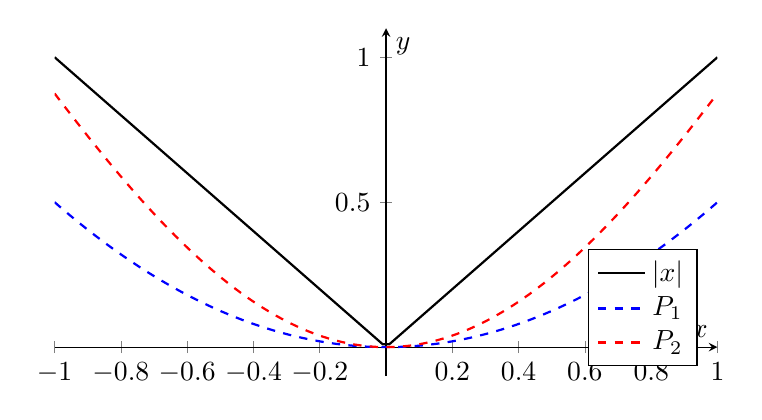
\begin{tikzpicture}
\begin{axis}[
    width=10cm, height=6cm,
    axis lines=middle,
    xlabel={$x$}, ylabel={$y$},
    domain=-1:1, samples=100,
    ymin=-0.1, ymax=1.1,
    legend pos=south east
]
\addplot[black, thick] {abs(x)};
\addplot[blue, thick, dashed] {0.5*x^2};
\addplot[red, thick, dashed] {0.5*x^2 + 0.5*(x^2 - (0.5*x^2)^2)};
\legend{$|x|$, $P_1$, $P_2$}
\end{axis}
\end{tikzpicture}
\end{center}

Each iteration pushes $P_n$ closer to $|x|$ from below. The correction term $\frac{x^2 - P_n^2}{2}$ is always non-negative (since $P_n \leq |x|$), so the sequence is increasing.

\section*{The key identity}

The hint gives: $|x| - P_{n+1}(x) = \bigl[|x| - P_n(x)\bigr] \cdot \left[1 - \frac{|x| + P_n(x)}{2}\right]$.

Let $e_n(x) = |x| - P_n(x)$ be the error. Then:
$$
e_{n+1} = e_n \cdot \left(1 - \frac{|x| + P_n}{2}\right).
$$

\section*{Two things to prove}

\textbf{1. $0 \leq P_n \leq P_{n+1} \leq |x|$ for $|x| \leq 1$:}

Since $P_n \leq |x| \leq 1$, we have $|x| + P_n \leq 2$, so the factor $1 - \frac{|x|+P_n}{2} \geq 0$. Combined with $e_n \geq 0$, we get $e_{n+1} \geq 0$, i.e.\ $P_{n+1} \leq |x|$. Also $P_{n+1} - P_n = \frac{x^2 - P_n^2}{2} = \frac{(|x|-P_n)(|x|+P_n)}{2} \geq 0$.

\textbf{2. The error goes to $0$ uniformly:}

Since $P_n \geq 0$, the factor $1 - \frac{|x| + P_n}{2} \leq 1 - \frac{|x|}{2}$. So:
$$
e_n(x) \leq |x| \cdot \left(1 - \frac{|x|}{2}\right)^n.
$$
Now maximize $g(u) = u(1 - u/2)^n$ over $u \in [0,1]$. Calculus (or the bound $(1-u/2)^n \leq e^{-nu/2}$ and optimizing $ue^{-nu/2}$) gives $\sup_u g(u) \leq \frac{2}{n+1}$.

So $\|P_n - |x|\|_\infty \leq \frac{2}{n+1} \to 0$. Uniform convergence!

\section*{Why this matters}

This gives a direct, constructive proof that $|x|$ can be uniformly approximated by polynomials --- without invoking the full Weierstrass theorem. Since $\max(f,g) = \frac{f+g+|f-g|}{2}$, this lets you build up approximations to any continuous function via the Stone--Weierstrass machinery.

\end{document}